\documentclass{article}
\usepackage[utf8]{inputenc}

\title{Malware Detection: Hands on}
\author{Francesco Piccinno}
\date{\today}

%\usepackage{natbib}
\usepackage{biblatex}

\usepackage{listings}
\usepackage{graphicx}
\usepackage{subfigure}
\usepackage{anysize}
\marginsize{3cm}{2cm}{1cm}{1cm}

\begin{document}

\maketitle

\section{What is malware?}

Malware is a generic term to indicate a generic malicious software or malicious code. Several authors attempted to provide a specific definition for the term malware. Christodorescu and Jha \cite{Christodorescu} describe a malware as software program whose objective is malevolent. McGraw and Morrisett \cite{mcf} instead classify a malware as any code added, changed or removed from a software system in order to intentionally subvert the intended functionality of the system. In this short report we consider the word ``malware'' a generic term that encompasses viruses, trojans, spywares and other intrusive code.

\section{Malware Detector}

A malware detection is a software component whose objective is to identify malwares. The detector attempt to help protect the system by detecting malicious behavior. But how a automatic component can understand what is malicious and what is not? In order to simplify, we can see a malware detector as a black box system that takes two inputs: the knowledge of the malicious behavior and the input program under inspection. How this ``knowledge base'' is built and which information is encoded within it characterize the detection tool.

There are essentially three techniques that are employed for malware detection:

\begin{description}
  \item[Signature based] Signature-based detection uses its characterization of what is known to be malicious to decide the maliciousness of a program under inspection.
  \item[Anomaly based] An anomaly-based detection technique uses its knowledge of what constitutes normal behavior to decide the maliciousness of a program under inspection.
  \item[Specification based] Specification-based techniques leverage some specification or rule set of what is valid behavior in order to decide the maliciousness of a program under inspection. Programs violating the specification are considered anomalous and usually, malicious.
\end{description}

Additionally, several sub-approaches are possible, irrespectively of the main technique being used. Namely there are static, dynamic and hybrid approaches. For example, using a static approach jointly with a signature-based detection would only leverage structural information of the file, such as specific sequence of bytes, in order to detect potentially harmful code. The dynamic approach will leverage runtime information, such as stack analysis or sequence of system calls invoked, trying to detect a malicious behavioral pattern. Hybrid techniques combine the two approaches. Figure \ref{fig:main} graphically sketch the context just described.

\subsection{Signature based detection} % (fold)
\label{sub:signature_based_detection}

Signature-based detection attempts to extract an unique feature or signature that match a known malware for its future detection. Ideally a signature should be enough to identify any piece of code or software exhibiting the malicious behavior encoded in the signature. A tool employing this technique must have access to a large repository of signatures and be able to detect all known malwares for which a signature is known. The main problem of this approach is the process of signature derivation mainly rely on human expertise, although some automatized solutions exists. Another big drawback is the fact that this malware detection solution cannot detect attacks for which a signature is not present (zero-day attacks).

% subsection signature_based_detection (end)

\subsection{Anomaly based detection} % (fold)
\label{sub:anomaly_based_detection}

To realize a malware detector employing the anomaly-based technique two phases are required. The training phase is used to let the tool ``learn'' what is the \emph{normal} behavior. The second phase, is the detection phase, in which the tool based on the knowledge acquired in the first phase, tries to detect potentially harmful programs. A key advantage of this detection technique is its ability to discover potential zero-day attacks or better attacks that are previously unknown to the malware detector. On the other hand there are two big limitations involving this procedure. The first one is is the complexity involved in determining which are the key features that should be extracted and processed in the learning phase. The second one is the high true-negative rate (a program classified as malicious although it is not). The problem is due to the approximation that the designer of the tool indirectly create during the training phase of the tool. Indeed a condition that is never met during the training phase that instead shows up during the monitor phase would produce a false alarm.
% subsection anomaly_based_detection (end)

\subsection{Specification based detection} % (fold)
\label{sub:specification_based_detection}

Specification-based detection was born as an attempt to address the high false alarm rate involved with anomaly-based detection techniques. In specification-based detection, the training phase can be thought as a derivation phase, whom aim is to extract a set of rules that describe all the valid behavior any software component can exhibit. Of course a complete and rich derivation of all the rules is a tedious and complex task. Indeed, for a quite large complex system, the complete and accurate specification of what is permitted and what can be intractable.
% subsection specification_based_detection (end)


\section{Examples from the Literature}

This section is dedicated to a brief overview of what we think are the most important and promising techniques for malware detection. The scope of this section is not to provide a complete review of all the possible solutions but just to highlight the common key concepts that have emerged from the study of this active research field.

\subsection{Anomaly based detection - Dynamic solutions}

In \cite{wang04raid-payl}, Wang and Stolfo presented PAYL. They presented a very simple mechanism for anomaly detection targeted to the protection of several network services for a system. For each service port the expected payload is calculated and a byte frequency distribution is then evaluated. This distribution allowed the construction of a \emph{centroid model} for each of the host's services. The authors then proposed to compare incoming payloads with the centroid model by measuring the Mahalanobis distance between the two. This distance takes into account the correlations of the data set and is scale-invariant therefore yielding a stronger statistical similarity measurement.

A complete different proposal is the one from Hofmeyr et al. \cite{Hofmeyr}, a work mainly targeted on the study of sequences of system call in order to detect malicious behaviors. First, a ``normal'' profile that represent the normal behavior of system's services is derived (n-gram based). An anomaly is then detected whenever a given system call sequence differs for more than a given threshold from the normal profile. Hamming distance is used as similarity measurement for comparing system call sequences.

Sekar et al. \cite{Sekar} proposed a similar approach based on a Finite State Automata. The change of state is driven by a syscall invocation. The training phase, which consists in the construction of the FSA is straightforward. Once a syscall is invoked a transition is added to the automaton. The resulting FSA represent the ``normal'' flow of the program. This knowledge is then exploited to track down possible abnormal sequence of syscall invocations. This method seems to have a lower false-positive rate than its counterpart based on n-grams.

A complete different approach based on statistical frequency analysis is the work of Sato et al. \cite{Sato}. The frequency of system calls is indeed used to extract a profile of a given program. The more frequent a given system call is used the lower is its ``ranking number'' in this profile. Once the profile has been established, the distance or similarity between the profile and sampled data is evaluated by using the a DP matching algorithm. The distance given by the matching algorithm serves as an indicator of the maliciousness of the program.

\subsection{Specification based detection - Dynamic approach}

Sekar et al. \cite{Sekar2} proposed a method to effectively conduct a live auditing of a given program. The key idea of the method is a translation process that takes in input the program and outputs an a representation of it in an custom language, called Auditing Specification Language. This ASL jointly with an infrastructure able to capture system calls being invoked, is then linked to the final program. The system call being intercepted are matched against the ASL code and if a mismatch is found the program is considered to be malicious.

A completely different approach, that bases its idea on the LIFO nature of how calls are invoked is the work from Lee et al \cite{lee}. The authors proposed an approach that seems to protect from most common stack smashing attacks. For this method to work correctly, the processor has to maintain its own stack, called a Secure Return Address Stack (SRAS). This structure is then used to detect possible control flow modification carried out by the malware.

\subsection{Specification based detection - Static approach}

Bergeron et al. proposed a novel approach for detecting maliciousness of an executable. By leveraging a static analysis and then by using a translation to an intermediate representation of the assembly code, a control flow graph of the executable is derived. Another derivation is then applied on the just constructed CFG graph. The output of this procedure is an API-graph where only API calls are considered. A set of security policies are then used to derive a critical API sub-graph, that is then evaluated for maliciousness.


\subsection{Specification based detection - Hybrid approach}

StackGuard \cite{Cowan} is the name of a product nowadays present in almost all the recent Linux distributions, that employs stack-canary techniques to protect the program again stack-smashing misuses. The product is a compiler extension that attempts to secure several routines valuated as unsafe (e.g. functions dealing with strings) by introducing a canary word before the return address. Any buffer overflow condition will result in an overwrite of the stack canary. This modification is detected before the actual malicious control flow modification takes place.

\subsection{Signature based detection - Static approach}

Sung et al. \cite{SAV} introduced a very interesting signature-based technique for detecting malicious programs in Windows environments. The signature is essentially a sequence of Windows API calls (n-grams). Each API call is a 32-bit number where the high 16-bits correspond to the module number, while the lower 16-bits are relative to the function being called. From a static inspection of the executable various sequences of API calls are extracted and compared with a database of known signatures. The similarity measurement in this case is the Euclidean distance.

\section{Our contribution}

As you will understand later, this work takes inspiration from the several proposed detection techniques presented in the previous section. Our contribution merely consists in the creation of a framework that let the analyzer experiment with the malware being inspected.

\subsection{Obtaining a behavioral description with Ether}

Initially, we thought on how to dynamically trace an unknown program in a isolated environment, in order to get a trace of its behavior. In order to maintain transparency during detection and at the same time to offer an isolated sandbox for analysis we focused our attention on virtualization technologies, mainly on Ether. Ether is a tool that allows malware analysis via hardware virtualization extensions, by using as base the XEN hypervisor. The tool is a research level software targeting the 3.1 version of XEN and offers interesting features such as syscall tracing, instruction level tracing, memory write detection and also a simple unpack-execution detection that is able to detect various packers.

Although the tool seems promising and complete in its feature set, the product is not using the current version of XEN code-base 4.1 and it is only supporting Windows XP SP2 guests (through hard-coded configuration parameters). Moreover the syscall tracing capabilities in which we were interested in is limited, in the sense that a live inspection of the stack of the program and of other parameters passed during syscall invocations is not possible at the current state.

\subsection{Dynamic binary instrumentation}

Due to the limitations of Ether, we decided to invest a little time to create a simple and effective syscall tracer that exploits dynamic binary instrumentation techniques. Although the final tool is not transparent and can be detected by the malware, we decided to go for it instead of investing a larger amount of time and effort to introduce the same functionalities in Ether (also because we were not sure about the outcome of the experiment).

In order to produce a ready to go tool, we used PIN a dynamic binary instrumentation framework that allows to quickly create dynamic program analysis tools. Indeed, by just leveraging the \texttt{PIN\_AddSyscallEntryFunction} we were able to detect all the syscall invocations in a given program. The functionality of the tracer was then improved in order to support a complete inspection of all parameters being passed to a given syscall invocation. To this end we have introduced a simple parser, that starting from Windows syscall definitions expressed in a series of \texttt{.h} header files was able to derive a automatic code whose objective was to log the contents of the variables being passed on the stack.

The tool also provide to the user the possibility of introducing custom code for in the middle of automatically generated code. This allows the creation of personalized function that focus their attention on certain syscall functions (e.g. we have used this mechanism to control the \texttt{DeviceIoControlFile} syscall and analyze TCP and UDP payloads), such as the one presented in Listing \ref{lst:hook}.

\begin{lstlisting}[language=C,caption={DeviceIoControlFile hooking},label=lst:hook]
if (IoControlCode == IOCTL_AFD_CONNECT)
{
  W::PAFD_CONNECT_INFO info = (W::PAFD_CONNECT_INFO)InputBuffer;

  /* ... */

  if (info->RemoteAddress.sa_family == AF_INET)
  {
    W::PSOCKADDR_IN sin4 = (W::PSOCKADDR_IN)&info->RemoteAddress;
    LOGFN("\t\tSOCKADDR RemoteAddress = \"\"\"%hu.%hu.%hu.%hu:%hu\"\"\"\n",
        (short)((sin4->sin_addr.s_addr >> 24) & 0xff),
        (short)((sin4->sin_addr.s_addr >> 16) & 0xff),
        (short)((sin4->sin_addr.s_addr >> 8) & 0xff),
      (short)(sin4->sin_addr.s_addr & 0xff), __htons(sin4->sin_port)
    );
  }
}
\end{lstlisting}

The core functionality of the tool are straightforward. The tool simply dynamically inspect the target program and intercept any syscall invocation. All the information are printed out in log file that can be analyzed later by the PyMal framework we developed.

\subsection{PyMal Framework}

The PyMal framework essentially consists of two basic component, the collector and the analyzer. The collector, as the name suggests, simply takes in input the log file produced in the first phase of analysis and extract all the possible information from it. The information being collected include full dump of any in/out parameters of the syscall (also complex \texttt{struct} s are supported), syscall number, syscall name, return code and the address of the caller (used for positional analysis).

The analyzer is instead a meta module that consists of several functions, ranging from n-gram statistical analysis to cosine-similarity metrics. It can be used as is or in a interactive way, thus allowing the user to express novel analysis techniques.

\subsection{Playground}

We used the tool to study several malwares with the final aim to find a common sequence of syscalls invocation that could be thought as malicious. Our idea is similar to the one proposed by Sung et al. \cite{SAV}. The difference resides in two main points. The first is that the analysis is focused only on syscalls instead of API calls. The reason resides in the fact that syscall analysis can be easily implemented at the VMM level (as Ether does by ) and it is very hard to detect.

The second key difference in our approach is the final goal. We were looking for a common signature or better sequence of syscalls that identify a give malware. We are not looking for modification of the control flow of a ``sane'' program due to exploitation condition, but focused our attention on malware identification.

\begin{table}[h]
\centering
\begin{tabular}{|l|l|}
\hline
	MD5 Digest & Name \\
\hline
	\texttt{0d8ff206e44059599747bc4ecf617240} & Allaple \\
	\texttt{fda80b705a0ca0e493e0c9a1409a6abd} & Blackhole-zeus \\
	\texttt{34a136aacdd2cc36fccd0debf930e4dc} & Dapato \\
	\texttt{573276121a2df24f277bd54958e8c5fd} & FakeAV \\
	\texttt{c059816a9e77113092f7c6adb2deeceb} & Gamaure \\
	\texttt{607b2219fbcfbfe8e6ac9d7f3fb8d50e} & Ramnit \\
	\texttt{bf53d17ace809cb3015eaed88a46d8aa} & SCKeyLog \\
	\texttt{9fbf1209b37ea58fa85851673c368f89} & SpyEye \\
	\texttt{dd9ebd92fc796eed8acba98d902933df} & Sub7 \\
	\texttt{d5c12fcfeebbe63f74026601cd7f39b2} & W32.Xpaj \\
	\texttt{7b7890cc2d35c552e1fedef71960b49f} & Zeus \\
\hline
\end{tabular}
\caption{Malware samples analyzed}
\label{tab:summary}
\end{table}

Table \ref{tbl:summary} present the malware we have analyzed in our experiment. During the experimentation phase, we analyzed each sample in an isolated Windows XP virtual machine by running each under our syscall tracer. The syscall invocation sequence was then extracted from each run and inserted in a database. From this timeline, we extracted a sequence of k-grams, with k varying from 1 to 7. We then used these ``k-timelines'' to derive a PDF graph. The graphs are presented in Figure \ref{fig:pdf} and Figure \ref{fig:pdf-nn}. The first figure shows the PDF of all syscalls that were invoked (also including nested syscalls that is a syscall invoked by another syscall) while the second figure just take in consideration the outermost syscalls.

\begin{figure}[ht]
	\centering
	\subfigure{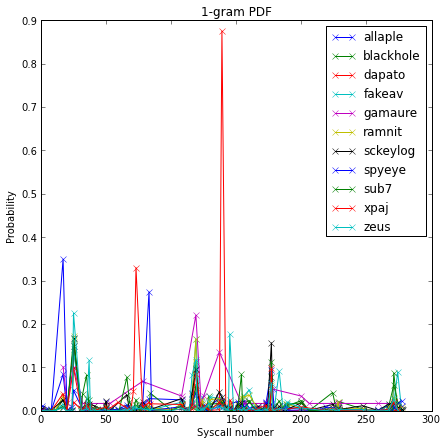
\includegraphics[width=0.49\textwidth]{1.png}}\hfill
	\subfigure{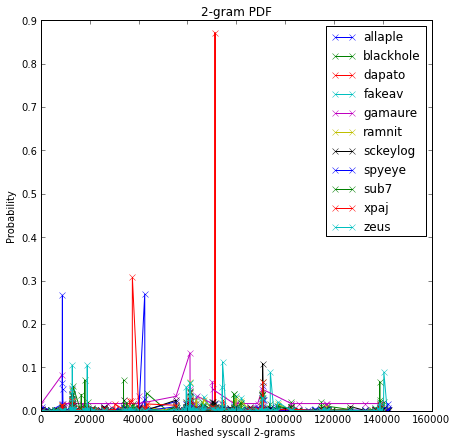
\includegraphics[width=0.49\textwidth]{2.png}}\\
	\subfigure{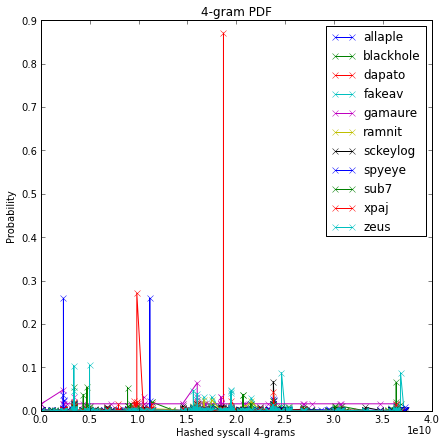
\includegraphics[width=0.49\textwidth]{4.png}}\hfill
	\subfigure{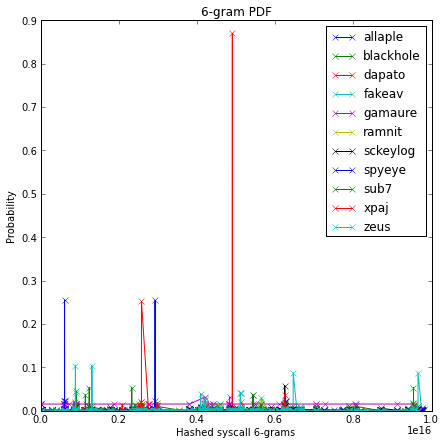
\includegraphics[width=0.49\textwidth]{6.png}}
	\caption{PDF with nested syscalls}
	\label{fig:subfigureExample}
\end{figure}

\begin{figure}[ht]
	\centering
	\subfigure{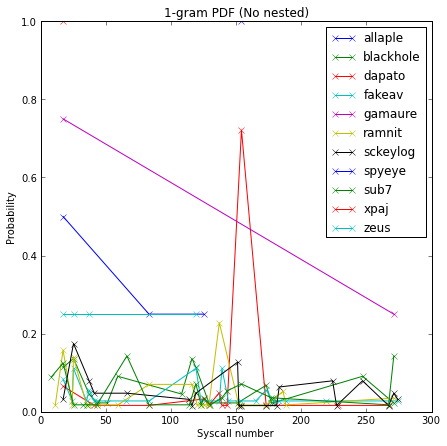
\includegraphics[width=0.49\textwidth]{n1.png}}\hfill
	\subfigure{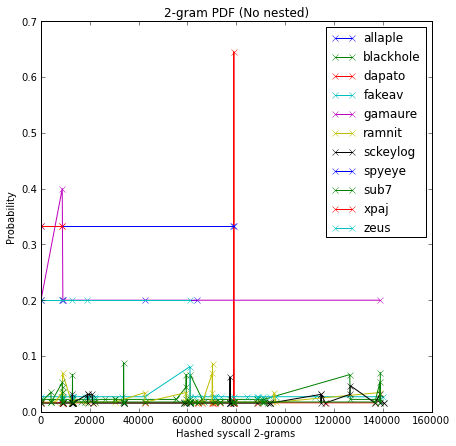
\includegraphics[width=0.49\textwidth]{n2.png}}\\
	\subfigure{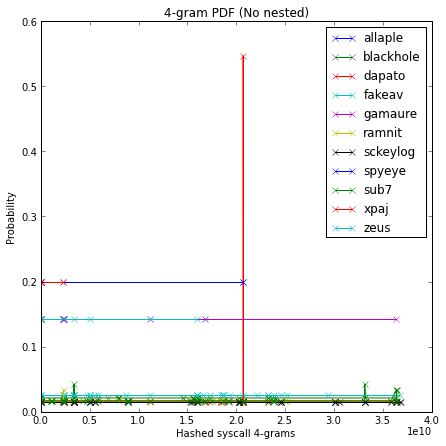
\includegraphics[width=0.49\textwidth]{n4.png}}\hfill
	\subfigure{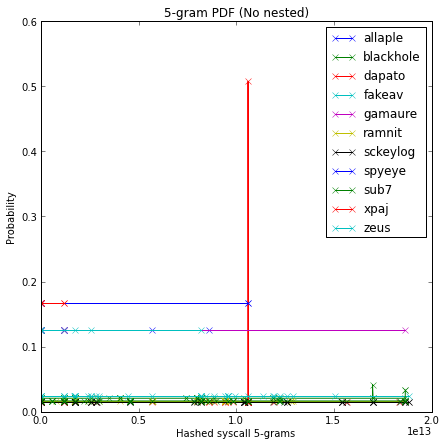
\includegraphics[width=0.49\textwidth]{n5.png}}
	\caption{PDF without nested syscalls}
	\label{fig:subfigureExample}
\end{figure}

The obtained results are not encouraging, in the sense that we were not able to find a commonality that could be used to track down malicious programs. This is somehow confirmed by the similarity measurements we get. Indeed by treating the k-gram sequence of syscalls as a multidimensional vector and evaluating the cosine similarity between various samples, as defined by the relationship \ref{eq:cos} we got almost complete match with similarity above 95\% percents for almost all the samples.

% \begin{equation}
% 	\label{eq:cos}
% 	\text{similarity} = \cos(\theta) = {A \cdot B \over \|A\| \|B\|} = \frac{ \sum\limits_{i=1}^{n}{A_i \times B_i} }{ \sqrt{\sum\limits_{i=1}^{n}{(A_i)^2}} \times \sqrt{\sum\limits_{i=1}^{n}{(B_i)^2}} }
% \end{equation}

Although we were not able to derive an automatized approach for malware identification, the tools we developed can be used for a preliminary analysis of an unknown program, leaving to the expertise of a human analyzer a deeper study of the sample.

To this end we briefly mention that the log can be easily parsed, in order to understand which files or pipes are used by a program, which modules are being loaded, which DNS queries are made or which packets are being exchanged between TCP or UDP endpoints. For example Listing \ref{lst:grep} shows some files being read by the zeus sample. In this case the malware is trying to extract passwords stored in Google Chrome web browser.

\begin{lstlisting}
$ grep "CreateFile): 0" -A 6 logs/* | grep ObjectName | sed -e 's/logs\/\([a-z0-9]*\)\.txt-.*"""\(.*\)"""/\1: \2/' | sort | uniq -c | grep -i "c\:"
  ...
  1 zeus: \??\C:\%APPDATA%\Google\Chrome\User Data\Default\Login Data
  1 zeus: \??\C:\%APPDATA%\Google\Chrome\User Data\Default\Login Data-journal
  1 zeus: \??\C:\%APPDATA%\Google\Chrome\User Data\Default\Web Data
  1 zeus: \??\C:\%APPDATA%\Google\Chrome\User Data\Default\Web Data-journal
  1 zeus: \??\C:\%APPDATA%\SharedSettings.ccs
  1 zeus: \??\C:\%APPDATA%\SharedSettings.sqlite
  1 zeus: \??\C:\%APPDATA%\SharedSettings_1_0_5.ccs
  1 zeus: \??\C:\%APPDATA%\SharedSettings_1_0_5.sqlite
  ...
\end{lstlisting}

Another possibility consists in deriving the FSM describing the syscall invocations being made by the program under inspection, as Sekar et al. proposed. The FSM can be then used to check for malicious variation of the behavior of the original program. To this end, you can take in consideration Figure \ref{fig:fsm} that depicts the FSM derivation of a simple program (Listing \ref{lst:simple}). The FSM on the left represents the safe execution while the second path represent the same program being abused to spawn a command interpreter.

digraph fsm {
	19 -> 299 [label=299];
	start -> 267 [label=267];
	234 -> 234 [label=234];
	234 -> 19 [label=19];
	267 -> 234 [label=234];
	299 -> 234 [label=234];
	start [style=bold];
}

digraph fsm {
	299 -> 399 [label=399];
	391 -> 50 [label=50];
	41 -> 266 [label=266];
	266 -> 182 [label=182];
	267 -> 234 [label=234];
	399 -> 50 [label=50];
	399 -> 399 [label=399];
	start -> 267 [label=267];
	50 -> 234 [label=234];
	50 -> 299 [label=299];
	50 -> 391 [label=391];
	182 -> 50 [label=50];
	182 -> 182 [label=182];
	217 -> 41 [label=41];
	234 -> 217 [label=217];
	234 -> 234 [label=234];
	start [style=bold];
}

\bibliographystyle{plain}
\bibliography{references}
\end{document}
